%\documentclass[a4paper]{article}
%% Language and font encodings
\documentclass[twocolumn,aps,prl]{revtex4-1}
\usepackage[utf8]{inputenc}
\usepackage[spanish, es-tabla]{babel}
\usepackage[T1]{fontenc}
\usepackage{amsmath}
\usepackage{siunitx}
\usepackage{multirow}
\usepackage{float}
\usepackage{enumitem} % enumerar

\sisetup{math-micro=\text{µ},text-micro=µ}

\usepackage[toc,page]{appendix}

%% Sets page size and margins
\usepackage[a4paper,top=2.4cm,bottom=2.4cm,left=0.5cm,right=0.5cm,marginparwidth=1.75cm]{geometry}

%% Sets caption text size(its bigger than text)
\usepackage{caption}
\captionsetup[figure]{font=small}
\usepackage{subcaption}

%% Useful packages
\usepackage{svg}
\usepackage{epstopdf}
\usepackage{amsmath}
\usepackage{graphicx}
% \usepackage[showframe]{geometry}% http://ctan.org/pkg/geometry
%\usepackage[colorinlistoftodos]{todonotes}
\usepackage[colorlinks=true, allcolors=blue]{hyperref}

\newcommand{\nstar}{n^*} 
\newcommand{\Nstar}{N^*} 

%%%%%%%%%%%%%%%%%%%%%%%%%%%%%%%%%%%%%%%%%%%%%%%%%%%%%%
%%%%%%%%%%%%%%%%%%%%%%%%%%%%%%%%%%%%%%%%%%%%%%%%%%%%%%
%%%%%%%%%%%%%%%%%%%%%%%%%%%%%%%%%%%%%%%%%%%%%%%%%%%%%%
%%%%%%%%%%%%%%%%%%%%%%%%%%%%%%%%%%%%%%%%%%%%%%%%%%%%%%
%%%%%%%%%%%%%%%%%%%%%%%%%%%%%%%%%%%%%%%%%%%%%%%%%%%%%%

\begin{document}

% ██   ██ ███████  █████  ██████
% ██   ██ ██      ██   ██ ██   ██
% ███████ █████   ███████ ██   ██
% ██   ██ ██      ██   ██ ██   ██
% ██   ██ ███████ ██   ██ ██████

\title{Práctico 1}
\author{M. G. Aramayo}
\affiliation{Matemática de sistemas biológicos, Instituto Balseiro}

% \begin{abstract}
% Mete acá las conclusiones.
% \end{abstract}

\maketitle


% ███████╗██╗  ██╗ ██╗
% ██╔════╝╚██╗██╔╝███║
% █████╗   ╚███╔╝ ╚██║
% ██╔══╝   ██╔██╗  ██║
% ███████╗██╔╝ ██╗ ██║
% ╚══════╝╚═╝  ╚═╝ ╚═╝

\section{Resolución Ej 1:}

Para este sistema discreto: 
$$n_{t+1} = f(n_t, K, r)= \frac{r n_t}{1+\frac{r-1}{K} n_t},$$ 

los puntos fijos $n^*$ se obtienen resolviendo la ecuación:
$$
n^* = f(n^*, K, r)
$$

Reemplazando:
$$
\nstar = \frac{r \nstar}{1+\frac{r-1}{K} \nstar}
$$


Resolvemos esta ecuación para $r\neq 1$ (donde hay dinámica):
$$
\nstar (r-1) (\nstar-K) = 0 \Rightarrow \left\lbrace ^{\nstar = K} _{\nstar = 0}  \right .
$$

Usando el siguiente criterio de estabilidad, proveniente de un análisis de pequeñas perturbaciones (Válido bajo las mismas hipótesis que permiten un desarrollo en series de Taylor), donde $n_{t+1} = f(n_t,r)$ representa el mapeo 1D y $\nstar$ el punto fijo a analizar:
$$
\begin{aligned}
|f_{n}\left(n^{*},r\right)| = |\lambda| &=\left\{\begin{array}{ll}
<1 & \text { Estable } \\
>1 & \text { Inestable } \\
=1 & \text { Marginalmente estable } \\
=0 & \text { Superestable }
\end{array}\right.
\end{aligned}
$$

Se obtiene que:
$$
|f_{n}\left(n^{*},r\right)|=\frac{K^{2} r}{(K+\nstar(r-1))^{2}}
$$

De analizar esta expresión (y analizar $r=0$ aparte), se obtiene lo que puede verse en la Fig. \ref{fig:estabilidad}.

%**********
\begin{figure}[ht!]
    \centering
    \begin{subfigure}[b]{0.3\linewidth}
        \centering
        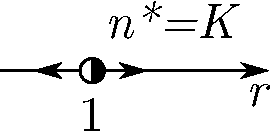
\includegraphics[width = 0.999\textwidth]{figuras/estabilidadK.pdf}
        \caption{}
        \label{fig:figuras/estabilidadK}
    \end{subfigure}\qquad\qquad\quad
    \begin{subfigure}[b]{0.3\linewidth}
        \centering
        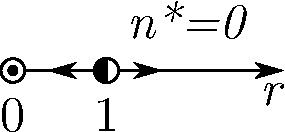
\includegraphics[width = 0.999\textwidth]{figuras/estable0.pdf}
        \caption{}
        \label{fig:figuras/estable0}
    \end{subfigure}\quad
    \caption{Estabilidad de los puntos fijos en según el parámetro $r$. El color negro indica el inicio de un intervalo de estabilidad y el blanco de un intervalo de inestabilidad. El círculo negro con marca blanca circular es un punto superestable.}
    \label{fig:estabilidad}
\end{figure}
%**********

En la Fig. \ref{fig:scripts/ex1} se tienen gráficos de los mapeos. Se observa que dentro de un intervalo de estabilidad $r$ controla la velocidad de crecimiento de la población. Hay dos casos particulares, si $r=1$ o $r=0$ no hay evolución y $n=0$, $n=n_0$ son sus respectivos puntos superestables. 

\begin{figure*}[ht!]  
    \centering
    % \begin{subfigure}[b]{0.33\linewidth}
        \centering 
        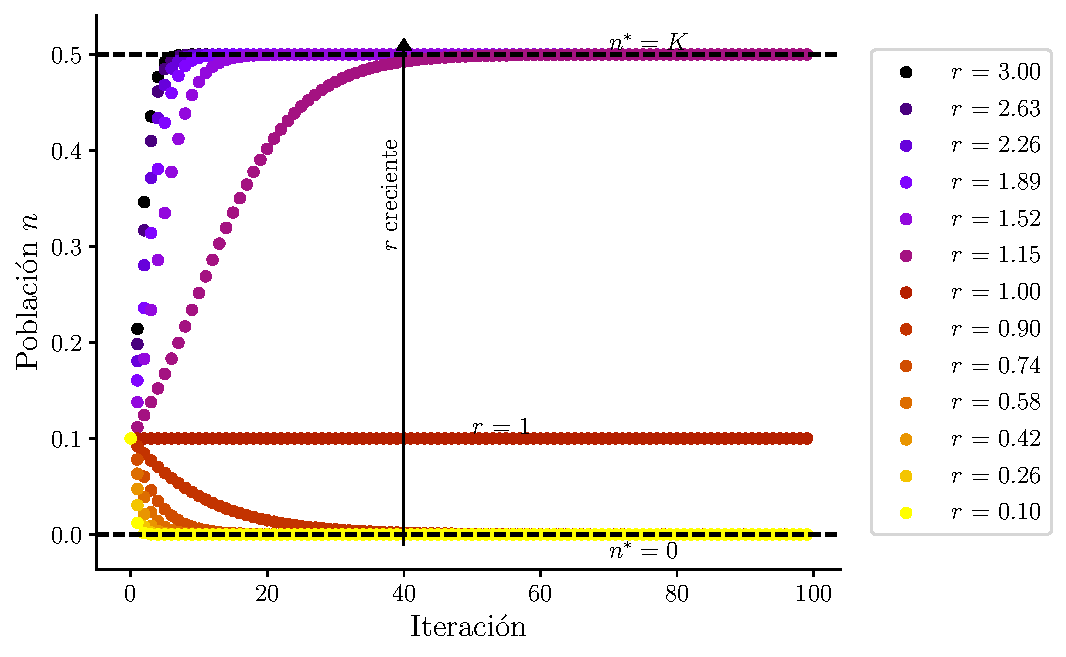
\includegraphics[width = 0.76\textwidth]{scripts/ex1.pdf}
        \caption{Gráfico del mapeo para distintos valores del parámetro $r$, los puntos fijos se indican con línea punteada. Hay un punto superestable cuando $r=1$, donde no hay dinámica. Se grafica con: $K = 0.5,N0 = 0.1$.}
        \label{fig:scripts/ex1}
    % \end{subfigure}\quad
\end{figure*}

% 
% ███████╗██╗  ██╗    ██████╗  
% ██╔════╝╚██╗██╔╝    ╚════██╗
% █████╗   ╚███╔╝      █████╔╝
% ██╔══╝   ██╔██╗     ██╔═══╝ 
% ███████╗██╔╝ ██╗    ███████╗
% ╚══════╝╚═╝  ╚═╝    ╚══════╝

\section{Resolución Ej 2:}

\begin{figure}[ht!]
    \centering
    % \begin{subfigure}[b]{0.45\linewidth}
        \centering
        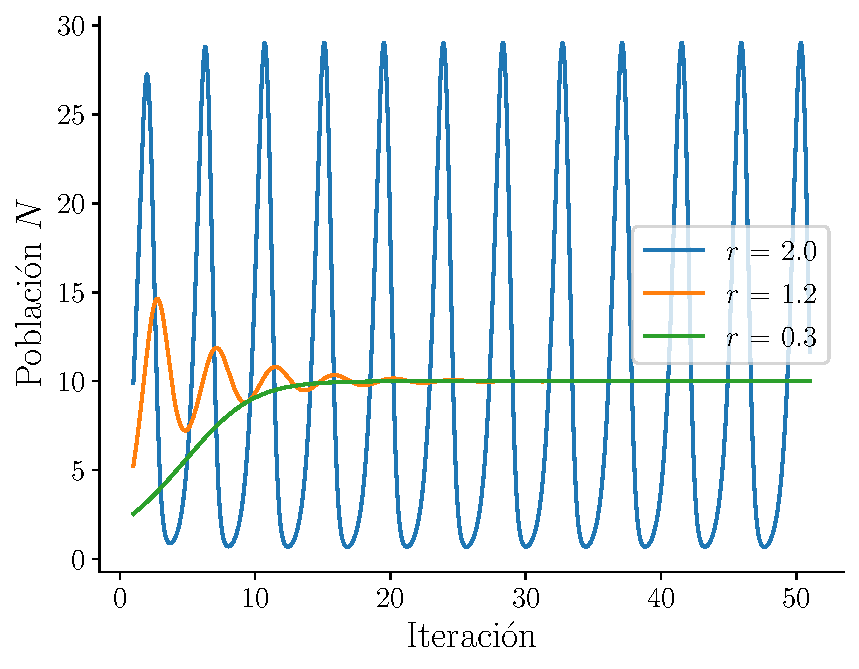
\includegraphics[width = 0.4\textwidth]{scripts/ex2-cosa.pdf}
        \caption{Soluciones de la ecuación logística con delay para tres valores del parámetro $r$.}
        \label{fig:scripts/ex2-cosa}
    % \end{subfigure}\quad
\end{figure}

\begin{figure*}[ht!]
    \centering
    % \begin{subfigure}[b]{0.33\linewidth}
        \centering
        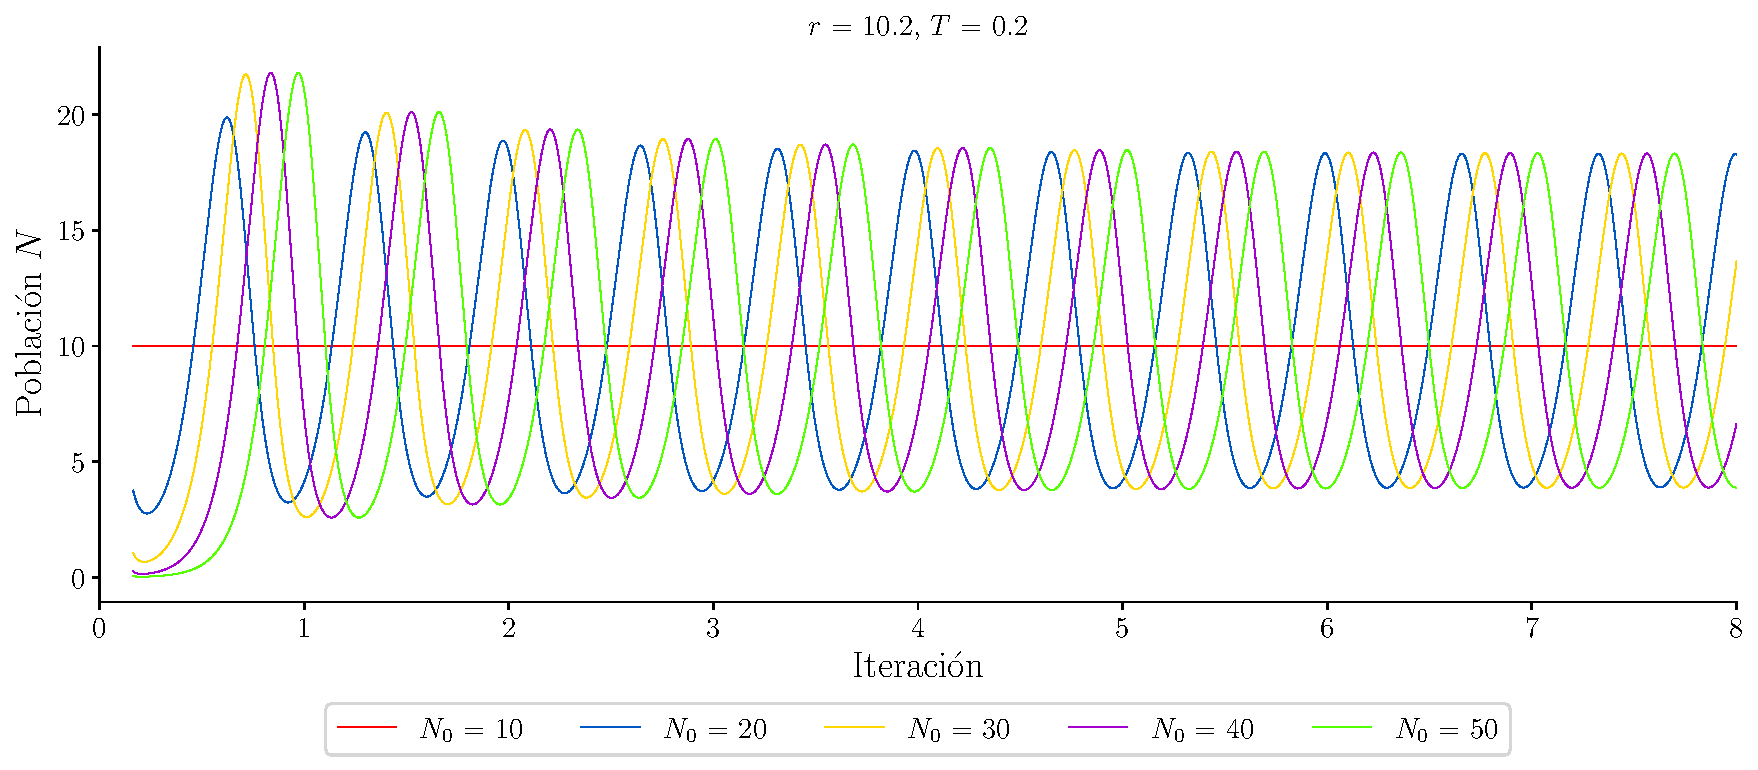
\includegraphics[width = 0.86\textwidth]{scripts/ex2-aprox.pdf} 
        \caption{Gráfico de soluciones ciclo límite para distintas condiciones iniciales.}
        \label{fig:scripts/ex2-aprox}
    % \end{subfigure}\quad
\end{figure*}

\begin{figure}[ht!]
    \centering
    % \begin{subfigure}[b]{0.33\linewidth}
        \centering
        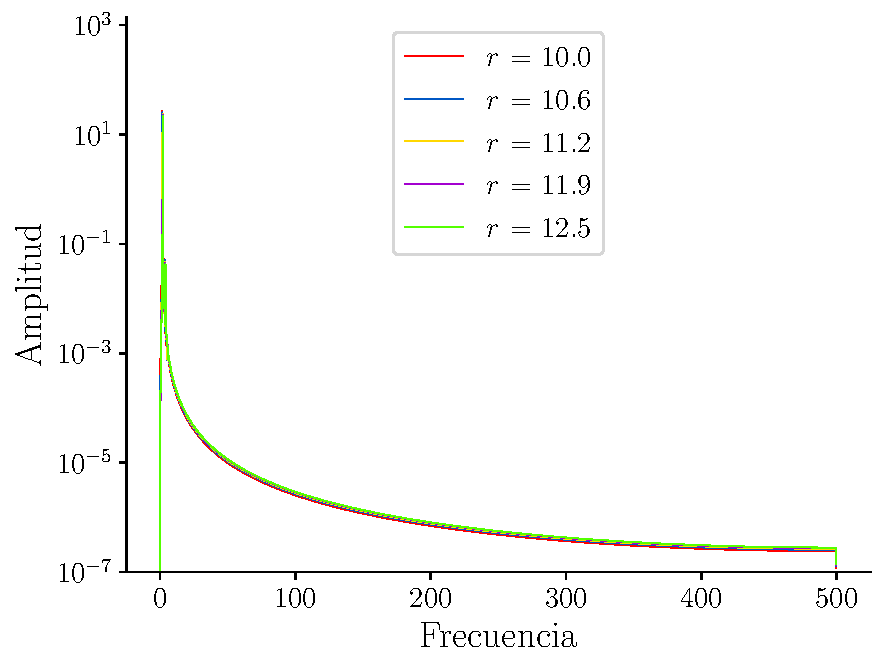
\includegraphics[width = 0.42\textwidth]{scripts/ex2-fourier-log.pdf}
        \caption{Transformada de Fourier del ciclo límite, para distintos valores de las condiciones iniciales.}
        \label{fig:scripts/ex2-fourier-log}
    % \end{subfigure}\quad
\end{figure}

\begin{figure*}[ht!]
    \centering
    % \begin{subfigure}[b]{0.33\linewidth}
        \centering
        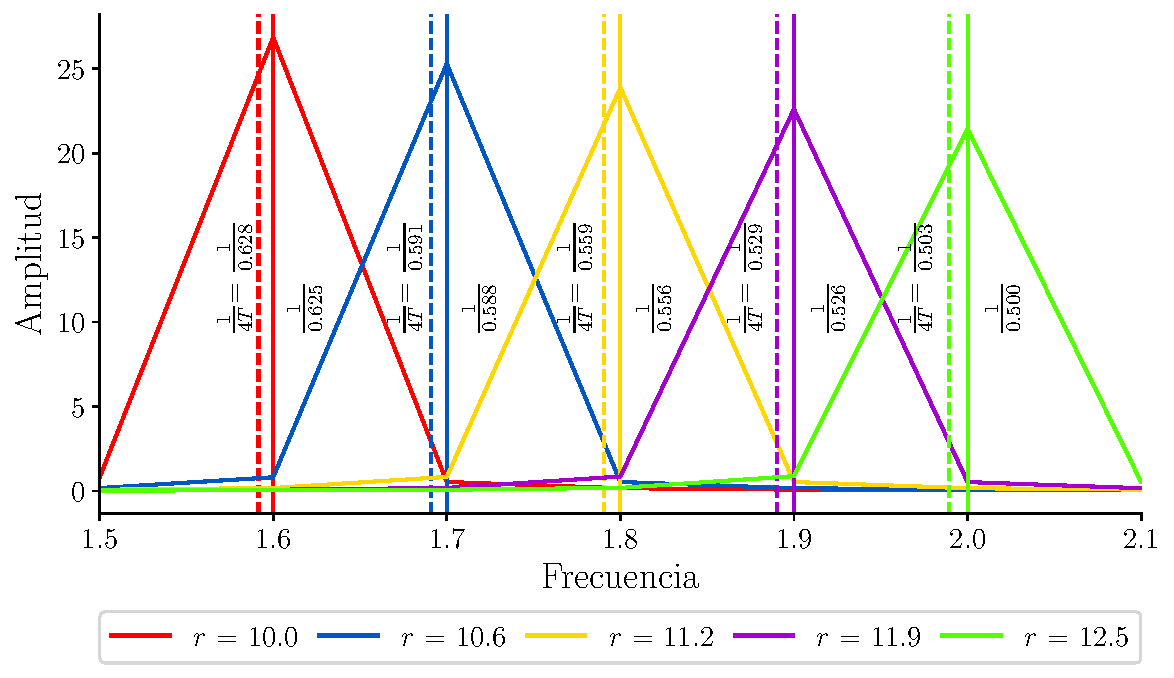
\includegraphics[width = 0.7\textwidth]{scripts/ex2-fourier-acotado.pdf}
        \caption{Transformada de Fourier del ciclo límite, en línea punteada esta la predicción teórica de la frecuencia de la señal. La línea continua es el valor obtenido de la transformada.}
        \label{fig:scripts/ex2-fourier-acotado}
    % \end{subfigure}\quad
\end{figure*}

\begin{figure*}[ht!]
    \centering
    % \begin{subfigure}[b]{0.33\linewidth}
        \centering
        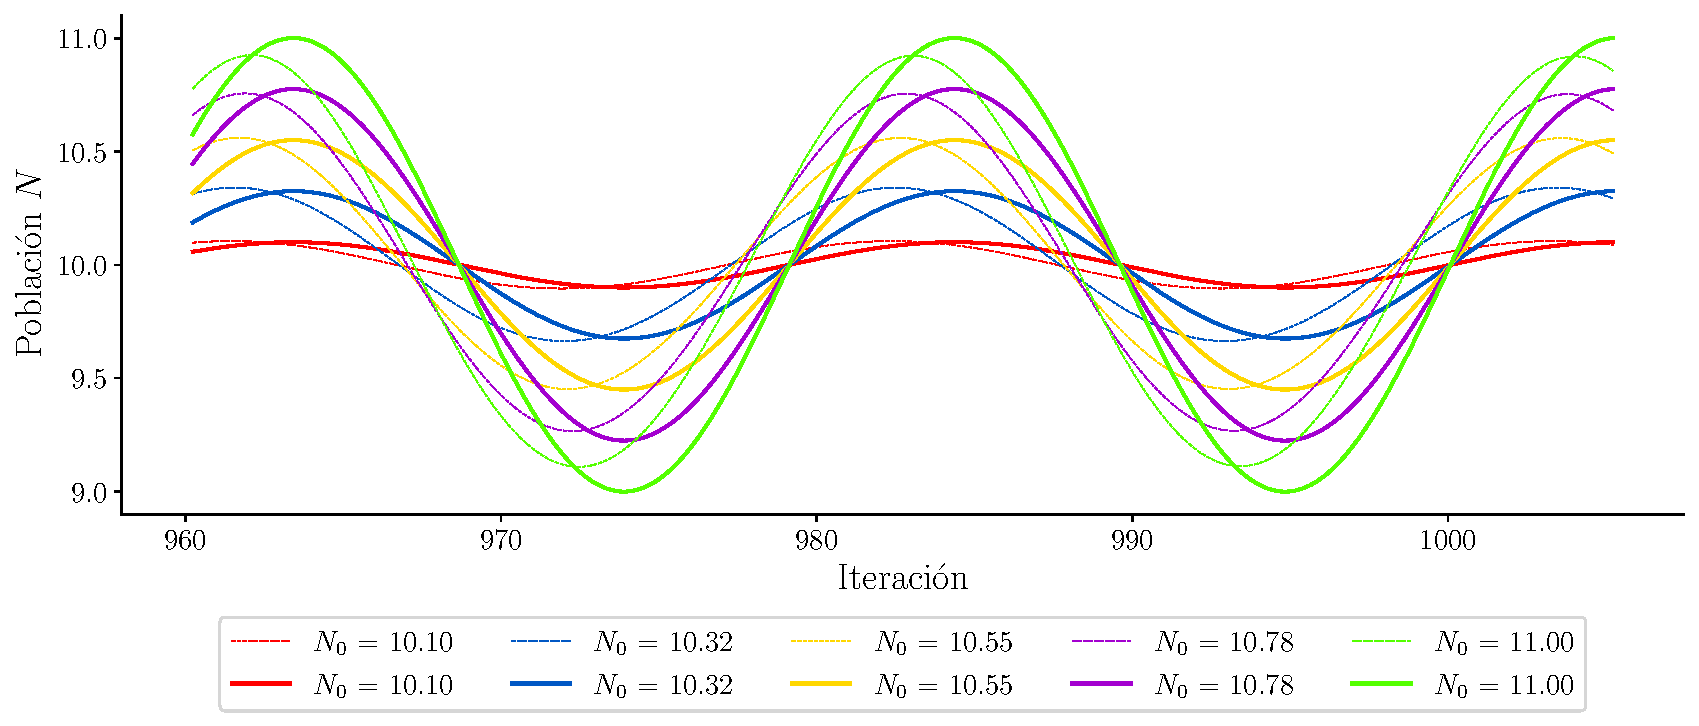
\includegraphics[width = 0.7\textwidth]{scripts/ex2-cosaPrueba.pdf}
        \caption{Gráficos de la aproximación analítica (línea continua) y solución numérica (línea discontinua) para valores de $N_0$ cercanos a $K$. Se grafica para $r = 0.3, K=10, \epsilon = 0.01$.}
        \label{fig:scripts/ex2-cosaPrueba}
    % \end{subfigure}\quad
\end{figure*}

En la Fig. \ref{fig:scripts/ex2-cosa} se tiene un gráfico de soluciones de la ecuación logística con delay. Están presentes los 3 regímenes de la ecuación logística con delay:
$$
\begin{array}{|l|l|}
\hline 0<r T <e^{-1} & \text { monótono } \\
e^{-1}<r T <\pi / 2 & \text { oscilatorio amortiguado } \\
\pi / 2<r T  & \text { ciclo límite } \\
\hline
\end{array}
$$

Por otro lado, bajo el régimen de ciclo límite se graficaron las soluciones a la ecuación logística con delay para distintas condiciones iniciales, se encuentran en la Fig. \ref{fig:scripts/ex2-aprox}. Puede observarse que la amplitud final no depende de la condición inicial para los parámetros elegidos.

Por otro lado, para obtener el periodo de oscilación del ciclo límite se graficó la transformada de Fourier que puede verse en la Fig. \ref{fig:scripts/ex2-fourier-log}. Se consideró como señal los puntos a $t>4$. En la Fig. \ref{fig:scripts/ex2-fourier-acotado} se tienen los periodos obtenidos a partir de la transformada de Fourier y las predicciones teóricas.

Además se graficaron en la Fig. \ref{fig:scripts/ex2-cosaPrueba} la solución de la ecuación logística con delay y de su cálculo mediante una aproximación analítica.

% 
% ███████╗██╗  ██╗    ██████╗     
% ██╔════╝╚██╗██╔╝    ╚════██╗    
% █████╗   ╚███╔╝      █████╔╝    
% ██╔══╝   ██╔██╗      ╚═══██╗    
% ███████╗██╔╝ ██╗    ██████╔╝    
% ╚══════╝╚═╝  ╚═╝    ╚═════╝     
%                                 
% 

\section{Resolución Ej 3:}

Sea $R(r)$ la función polinomios:
\begin{equation}\label{eqn:etiqueta1}
    R(r) = r^{k+1} 
        - \left( 
            r^k f_0 
            - \sum_{l=1}^k 
            \left( 
            r^{k-l} f_l \prod_{j=0}^{l-1} s_j  
            \right) 
        \right)
\end{equation}

tal que $R(1)=R$. Puede verse que:
\begin{equation}\label{eqn:etiqueta2}
    R(0) = - f_k \cdot  s_{k-1} \cdot \ldots \cdot s_{0}
\end{equation}

Como es sabido, se cumple $f_j \geq 0, \forall \in \lbrace 0, \ldots, k \rbrace$, y sobre la supervivencia $  0 < s_j < 1, \forall \in \lbrace 0, \ldots, k - 1 \rbrace$.

Si se cumple que $f_k > 0$ se tiene que $R(0) < 0$. 

$R$ es un polinomio y por tanto una función continua. Por esto tiene tantos cambios de signo en su valor a lo largo de $r$ como raíces tenga $R$. 

El criterio de Descartes indica que esta raíz es positiva y hay solo una, sea $r_1$ esta raíz. Como hay una única raíz hay un único cambio de signo en $R$ respecto a $r$ en la recta real. 

Si se tiene que $R(0)$ y $R(1)$ son negativos y $r_1>0$, se tiene que el cambio de signo ocurre después de estos valores. Es decir, la raíz no puede estar entre 0 y 1 porque eso implica que hay más de un cambio de signo (uno para ir de $R(0)$ negativo a positivo y otro para volver al negativo en $R(1)$) como esto no es posible por el criterio de Descartes se tiene que $r_1>1$.

% 
% ███████╗██╗  ██╗    ██╗  ██╗
% ██╔════╝╚██╗██╔╝    ██║  ██║
% █████╗   ╚███╔╝     ███████║
% ██╔══╝   ██╔██╗     ╚════██║
% ███████╗██╔╝ ██╗         ██║
% ╚══════╝╚═╝  ╚═╝         ╚═╝
%                             
% 

\section{Resolución Ej 4:}

Se grafican en la Fig. \ref{fig:scripts/ex4} del mapeo con distintas semillas de números aleatorios. Las secuencias aleatorias de $r$ produce un rango amplio de máximos de población. Una secuencia de valores altos de $r$ producen poblaciones enormes. Asimismo una racha de valores bajos resulta en la extinción de la población.

%**********
\begin{figure}[ht!]
    \centering
    % \begin{subfigure}[b]{0.33\linewidth}
        \centering
        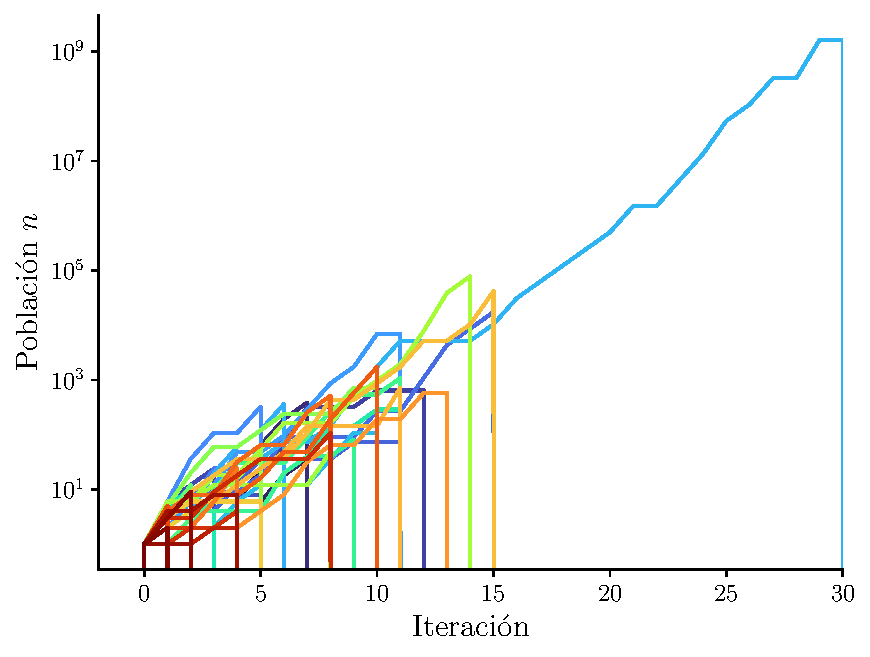
\includegraphics[width = 0.4\textwidth]{scripts/ex4.pdf}
        \caption{Gráficos del mapeo con distintas semillas de números aleatorios. Una secuencia específica de valores de $r$ produce un rango amplio de máximos de población.}
        \label{fig:scripts/ex4}
    % \end{subfigure}\quad
\end{figure}
%**********

% 
% ███████╗██╗  ██╗    ███████╗
% ██╔════╝╚██╗██╔╝    ██╔════╝
% █████╗   ╚███╔╝     ███████╗
% ██╔══╝   ██╔██╗     ╚════██║
% ███████╗██╔╝ ██╗    ███████║
% ╚══════╝╚═╝  ╚═╝    ╚══════╝
%                             
% 

\section{Resolución Ej 5:}

%**********
\begin{figure*}[ht!]
    \centering
    \begin{subfigure}[b]{0.495\linewidth}
        \centering
        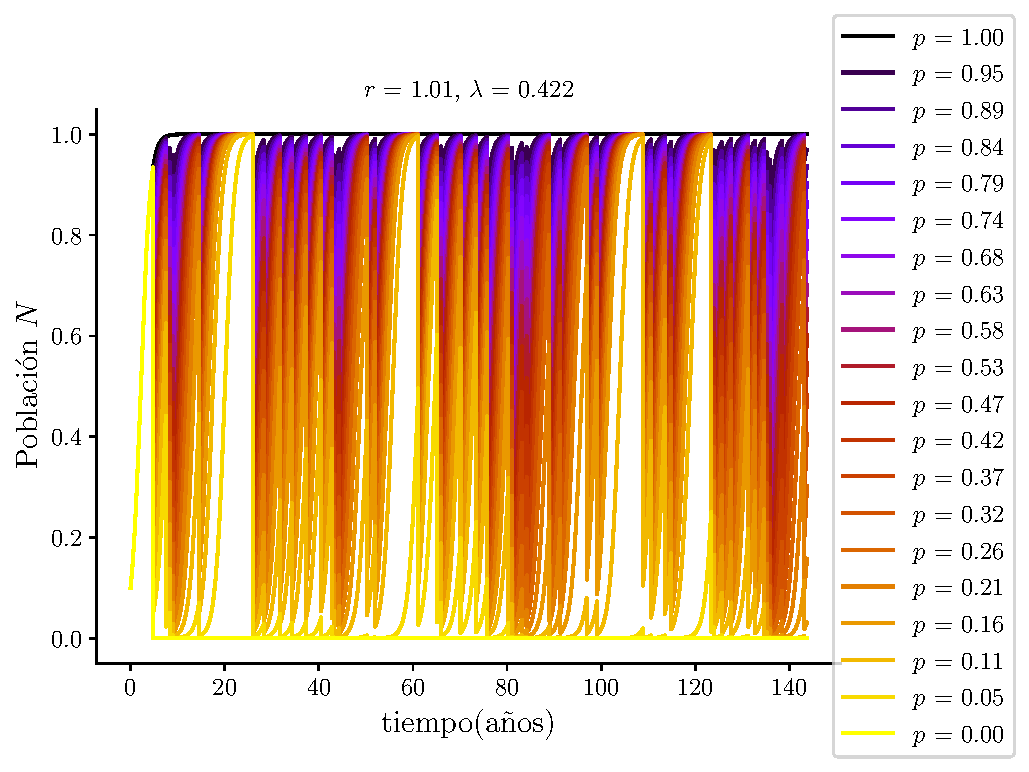
\includegraphics[width = 0.999\textwidth]{scripts/plots/ex5-02.pdf}
        \caption{}
        \label{fig:scripts/plots/ex5-02}
    \end{subfigure}
    % \quad
    \begin{subfigure}[b]{0.495\linewidth}
        % \centering
        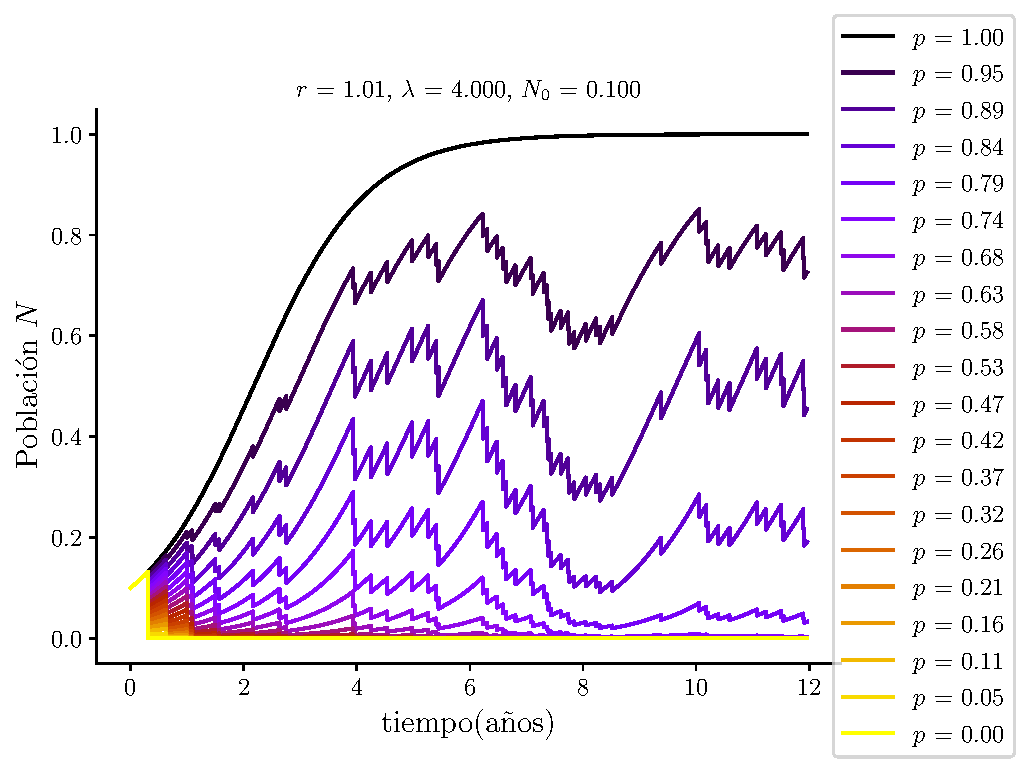
\includegraphics[width = 0.999\textwidth]{scripts/plots/ex5-19.pdf}
        \caption{}
        \label{fig:scripts/plots/ex5-19}
    \end{subfigure}
    \caption{Gráfico del modelo logístico interrumpido por desastres para distintos valores de $p$. Para cada valor de lambda se sigue la misma secuencia de desastres.}
    \label{fig:scripts/plots/ex5}
\end{figure*}
%**********

Utilizando un modelo logístico interrumpido por desastres que perturban la solución con un parámetro $p$ tal que: $N(t^+)=pN(t)$. Con un tiempo medio entre desastres $1/\lambda$. Se resolvieron las ecuaciones para 20 valores distintos de $p$, en dos casos: $r = \text{1.01}, \lambda = \text{0.422}$ en Fig. \ref{fig:scripts/plots/ex5-02} (Caso a) y $r = \text{1.01}, \lambda = \text{0.422}$ \ref{fig:scripts/plots/ex5-19} (Caso b). Dentro de cada caso se utiliza la misma secuencia de eventos desastrosos para comparar el efecto del parámetro $p$. En ambos casos se resolvió para 50 eventos desastrosos. 

Respecto a la dinámica se observó en el caso b que a medida que $p$ baja, la posibilidad de completar el crecimiento baja y la población empieza a crecer por debajo del punto fijo $K$. Se torna complicada la recuperación, para el caso a se observa que de las 20 curvas consideradas solo las 5 con el valor de $p$ más alto sobreviven, en el resto de casos se llegó a una extinción. 
En el caso b el tiempo medio de desastres $\lambda$ es más corto que el tiempo de recuperación $1/r$, para este caso todos los valores de $p$ intentados se encuentran por debajo de $K$. Esto no ocurre en el caso a donde el tiempo medio de la ecuación logística es más corto que el de la ocurrencia de desastres, por lo que la población se recupera hasta el valor $K$ para 16 de los 20 valores de $p$ considerados. Con esto en cuenta, es posible que el sistema se recupere si $1/r > 1/\lambda$. Esto depende de $p$ porque aun para el caso a se observa una extinción en estas condiciones para $p =\text{0.05}$.

% 
% ███████╗██╗  ██╗     ██████╗ 
% ██╔════╝╚██╗██╔╝    ██╔════╝ 
% █████╗   ╚███╔╝     ███████╗ 
% ██╔══╝   ██╔██╗     ██╔═══██╗
% ███████╗██╔╝ ██╗    ╚██████╔╝
% ╚══════╝╚═╝  ╚═╝     ╚═════╝ 
%                              
% 

\section{Resolución Ej 6:}

Para este sistema continuo:
\begin{equation}\label{eqn:Alle}
\frac{d N}{d t} =r N\left[1-\frac{N}{K}\right]\left[\frac{N}{A}-1\right] = f(N, K, r, A)
\end{equation}
$$
\frac{d N}{d t} = f(N, K, r, A) \qquad r>0, K>0 , A>0
$$

es conocido que los puntos fijos $N^*$ son las soluciones a la ecuación:
\begin{equation}\label{eqn:etiqueta3}
    0 = f(N^*, K, r, A), r>0, K>0, A >0
\end{equation}

Resolvemos esta ecuación para $r\neq 1$ (donde hay dinámica):
\begin{equation}\label{eqn:etiqueta3}
    - r \Nstar  (1 - \frac{\Nstar}{K}) (1 - \frac{\Nstar}{A}) = 0 \Rightarrow \left\lbrace ^{\Nstar = K, \Nstar = A} _{\Nstar = 0, }  \right .
\end{equation}

Usando el siguiente criterio de estabilidad, proveniente de un análisis de pequeñas perturbaciones (Válido bajo las mismas hipótesis que permiten un desarrollo en series de Taylor), donde $\frac{dN}{dt} = f(N, K, r, A)$ representa el sistema dinámico y $\Nstar$ el punto fijo a analizar:
$$
\begin{aligned}
    \frac{d f\left(x^{*}, r\right)}{d x} &=\left\{ 
        \begin{array}{ll}
            <0 & \text { Estable } \\
            >0 & \text { Inestable }
        \end{array}\right.
\end{aligned}
$$

Se tiene en este caso 3 puntos fijos, pero hay 2 que provienen de dos binomios similares pero con un parámetro distinto, los puntos fijos son los ceros de la función.

Para $\frac{d f\left(x^{*}, r\right)}{d x} (0):$ 
$$
\frac{d f\left(x^{*}, r\right)}{d x} (0) = -r \Rightarrow \text{Estable}
$$ 

Para $\frac{d f\left(x^{*}, r\right)}{d x} (A):$ 
$$
\frac{d f\left(x^{*}, r\right)}{d x} (A) = \frac{r}{K} (K-A)  
\left\lbrace
^{ K<A \Rightarrow \text{Estable}}
_{ K>A \Rightarrow \text{Inestable}} \right.
$$ 

Para $\frac{d f\left(x^{*}, r\right)}{d x} (K):$ 
$$
\frac{d f\left(x^{*}, r\right)}{d x} (K) = \frac{r}{A} (A-K) 
\left\lbrace ^{ K>A \Rightarrow \text{Estable}}
_{ K<A \Rightarrow \text{Inestable}} \right.
$$ 

En la Fig. \ref{fig:scripts/plots/ex6-y0chico02} se puede ver que para condiciones iniciales superiores a $A$ la población decrece hasta $A$, un punto fijo estable. Para valores de $A$ menores a $K$, el punto fijo resulta en $A$.

En la Fig. \ref{fig:scripts/plots/ex6-y0grande02} para condiciones iniciales entre 0 y $K$. Para un mismo r, a valores $A$ menores a $N_0$ el sistema tiende a $K$. A valores de $A$ mayores a $N_0$, la población decrece a 0. 

De ejemplos anteriores, el parámetro $r$ solo controla la rapidez con la que se llega a los puntos fijos. Pero no altera la estabilidad.

%**********
\begin{figure*}[ht!]
    \centering
    \begin{subfigure}[b]{0.495\linewidth}
        \centering
        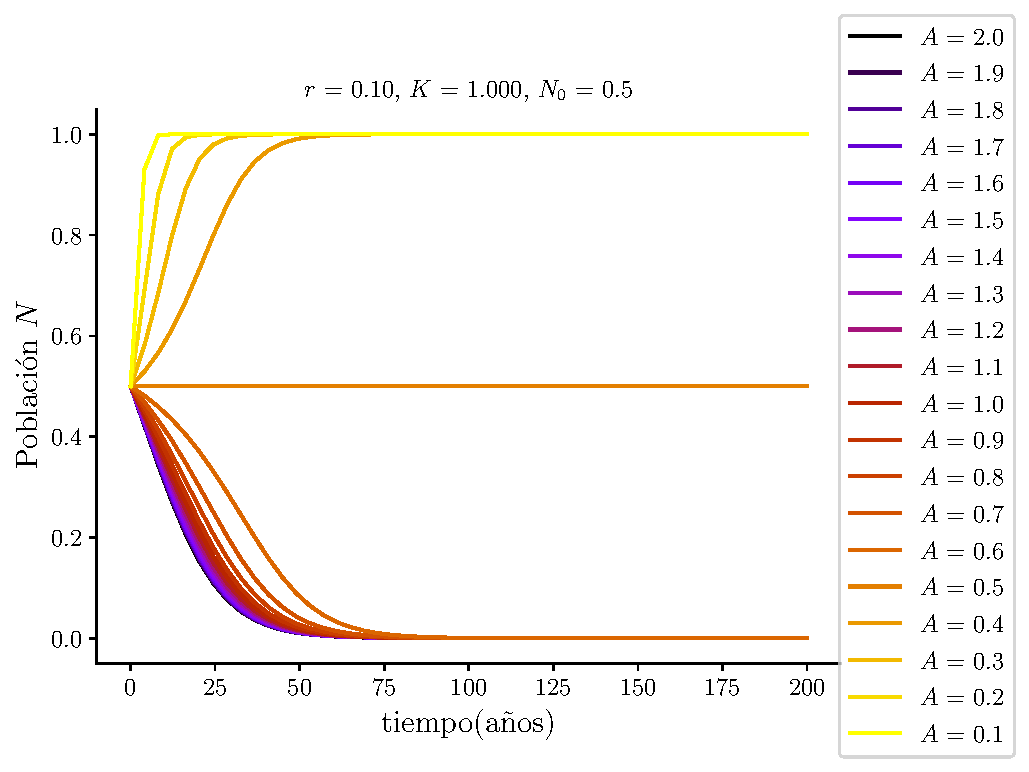
\includegraphics[width = 0.999\textwidth]{scripts/plots/ex6-y0chico02.pdf}
        \caption{}
        \label{fig:scripts/plots/ex6-y0chico02}
    \end{subfigure}
% \end{figure*}
% \begin{figure*}[ht!]
    % \centering
    \begin{subfigure}[b]{0.495\linewidth}
        \centering
        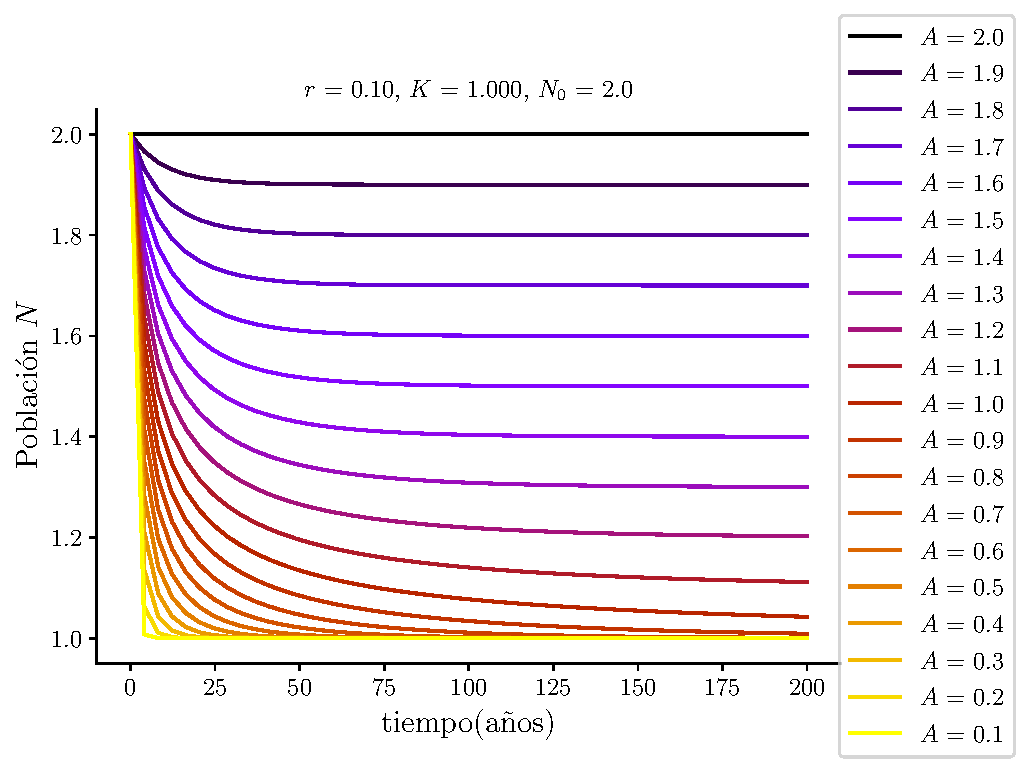
\includegraphics[width = 0.999\textwidth]{scripts/plots/ex6-y0grande02.pdf}
        \caption{}
        \label{fig:scripts/plots/ex6-y0grande02}
    \end{subfigure}
    \caption{Gráficos de la solución de la Ec. \ref{eqn:Alle} para $r=0.1$ y distintos valores de $A$. Por la naturaleza de uno de los puntos fijos, solo pueden verse para condiciones iniciales mayores a K.}
\end{figure*}
%**********

\bibliography{sample}

\end{document}
